% Shared content and layout for the main CV.
% The entry-point file defines \CVFontSetup.
\documentclass[10pt,a4paper]{article}

\usepackage[a4paper,left=0.46in,right=0.46in,top=0.43in,bottom=0.43in]{geometry}
\usepackage{fontspec}
\usepackage{graphicx}
\usepackage{array}
\usepackage{tabularx}
\usepackage{enumitem}
\usepackage{xcolor}
\usepackage{hyperref}
\usepackage{eso-pic}

\CVFontSetup

\definecolor{navy}{HTML}{17365D}
\definecolor{text}{HTML}{1E2630}
\definecolor{muted}{HTML}{586574}
\definecolor{rule}{HTML}{AAB7C4}
\definecolor{link}{HTML}{245A92}

\hypersetup{
  colorlinks=true,
  urlcolor=link,
  linkcolor=link,
  pdfauthor={Haotian Liu},
  pdftitle={Haotian Liu - Academic CV},
  pdfsubject={Academic CV for Japanese SGU master's applications}
}

\pagestyle{empty}
\setlength{\parindent}{0pt}
\setlength{\parskip}{0pt}
\setlength{\tabcolsep}{0pt}
\setlength{\emergencystretch}{1.5em}
\newcolumntype{Y}{>{\raggedright\arraybackslash}X}

\newcommand{\cvsection}[1]{%
  \vspace{5.8pt}%
  {\sffamily\bfseries\fontsize{10.8}{12.5}\selectfont\color{navy}\MakeUppercase{#1}}\par
  \vspace{1.5pt}%
  {\color{rule}\hrule height 0.6pt}\vspace{4.0pt}%
}

\newcommand{\entrytitle}[2]{%
  \begin{tabularx}{\linewidth}{@{}Y r@{}}
    {\sffamily\bfseries\fontsize{9.45}{11.4}\selectfont #1} &
    {\sffamily\fontsize{9.0}{11.4}\selectfont\color{muted} #2} \\
  \end{tabularx}\par
}

\newcommand{\entryrole}[1]{%
  {\itshape\fontsize{9.1}{11.3}\selectfont\color{muted}#1}\par\vspace{0.9pt}%
}

\newcommand{\publication}[3]{%
  {\fontsize{9.1}{11.3}\selectfont\textbf{#1}\par}%
  {\fontsize{9.1}{11.3}\selectfont
  \begin{tabularx}{\linewidth}{@{}Y>{\raggedleft\arraybackslash}p{1.12in}@{}}
    #2 & #3 \\
  \end{tabularx}}%
  \vspace{1.2pt}%
}

\newenvironment{cvitems}{%
  \begin{itemize}[
    label=\textbullet,
    leftmargin=11.5pt,
    labelsep=4.4pt,
    itemindent=0pt,
    topsep=0.3pt,
    partopsep=0pt,
    parsep=0pt,
    itemsep=2.8pt
  ]
  \fontsize{9.5}{11.9}\selectfont
}{\end{itemize}\vspace{2.5pt}}

\begin{document}
\color{text}
\fontsize{9.5}{11.9}\selectfont

% Paint the portrait in the page foreground so font metrics cannot move or
% suppress it. The coordinates align it with the top and right text margins.
\AddToShipoutPictureFG*{%
  \AtPageUpperLeft{%
    \put(\LenToUnit{\dimexpr\paperwidth-0.46in-0.80in\relax},\LenToUnit{-1.56in}){%
      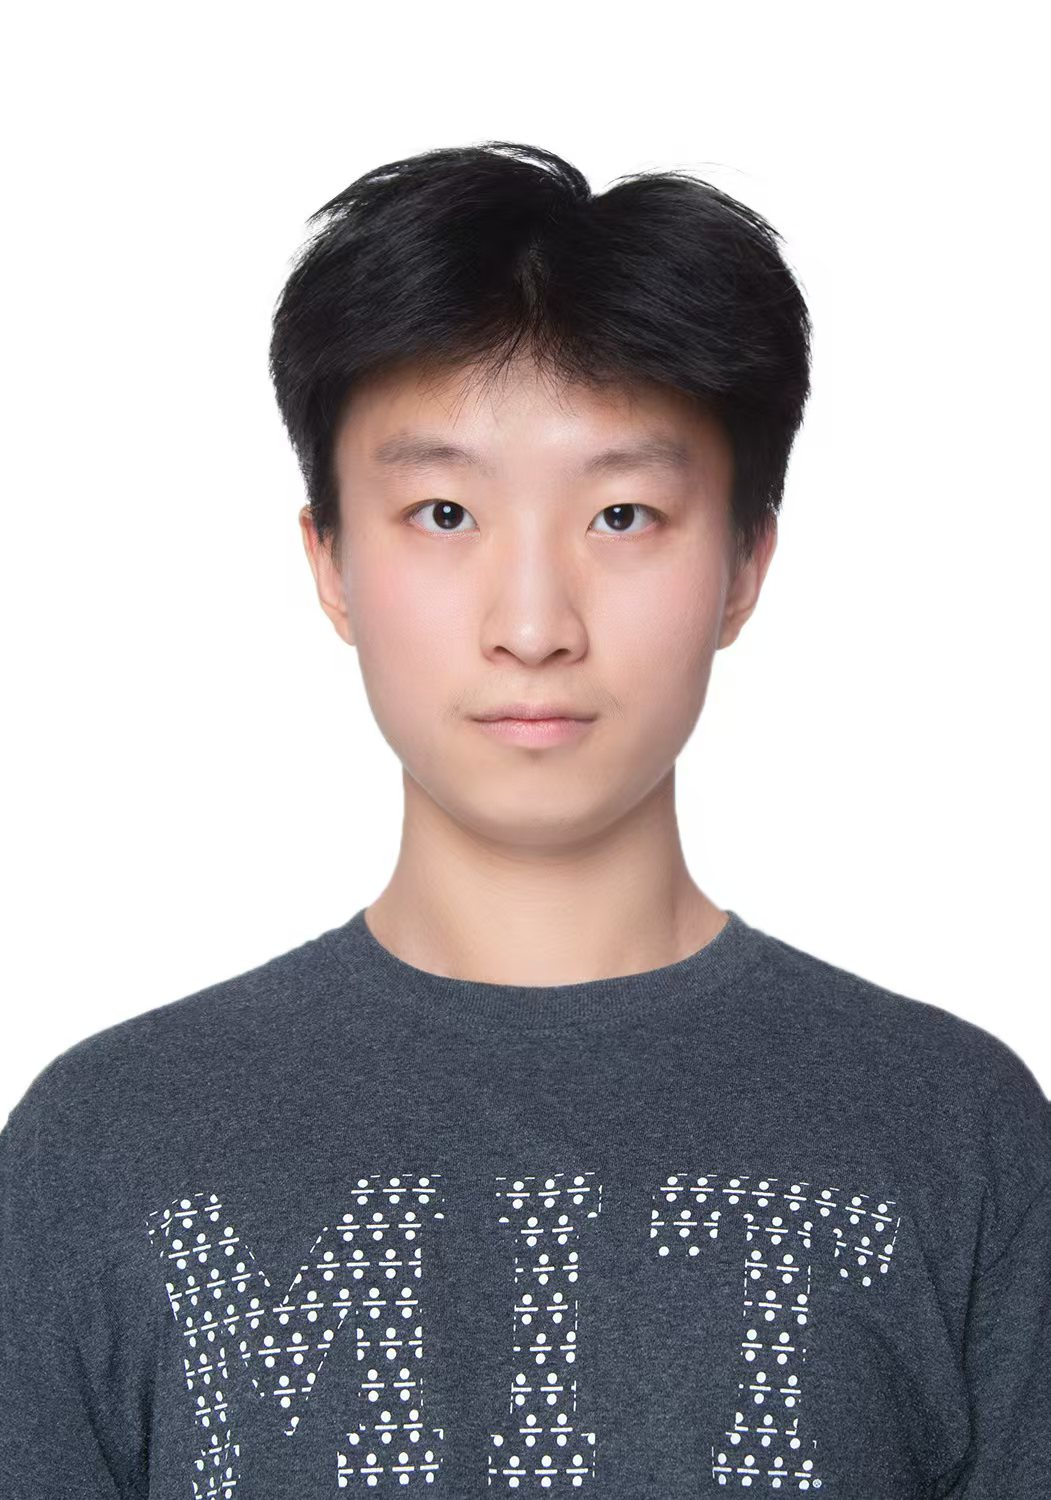
\includegraphics[width=0.80in,height=1.13in,trim=185 470 185 65,clip]{Haotian.jpg}%
    }%
  }%
}

% The left column is taller than the portrait, so the image no longer creates
% an empty header block. Full-width flow resumes immediately after Education.
\begin{minipage}[t]{\dimexpr\linewidth-1.08in\relax}
  \vspace{0pt}
  {\sffamily\bfseries\fontsize{22}{24}\selectfont\color{navy}Haotian Liu}\par
  \vspace{3.6pt}
  {\sffamily\fontsize{9.1}{11.5}\selectfont
    \href{mailto:haotianliu.me@gmail.com}{haotianliu.me@gmail.com}
    \enspace\textcolor{muted}{|}\enspace
    \href{https://haotian-io.github.io/}{Homepage}
    \enspace\textcolor{muted}{|}\enspace
    \href{https://github.com/haotian-io}{GitHub}
    \enspace\textcolor{muted}{|}\enspace
    \href{https://scholar.google.com/citations?user=hemBmosAAAAJ\&hl=en}{Google Scholar}}

  \cvsection{Education}
  \entrytitle{Xiamen University (XMU), Xiamen, China}{Sep. 2023 -- Jun. 2027 (expected)}
  \entryrole{B.Eng. in Software Engineering \textbar{} Overall Average: 82.50/100}
  {\fontsize{9.1}{11.3}\selectfont
  \textbf{Relevant Coursework:} Machine Learning for Decision-Making and Optimization (96); Algorithms for Modern AI (94); Introduction to Artificial Intelligence (93); Interactive Design (90); Data Warehouse (90).}
\end{minipage}

\cvsection{Publications}
\publication
  {PilotBench: A Benchmark for General Aviation Agents with Safety Constraints.}
  {\textit{IJCNN 2026}, \textbf{accepted}. Co-first author.}
  {\href{https://arxiv.org/abs/2604.08987}{arXiv:2604.08987}}
\publication
  {Long-Horizon Memory Governance for LLM Agents.}
  {\textit{Under review at EMNLP 2026.} First author.}
  {}
\publication
  {ProcuraClaw: Context-Aware Procurement Search via Adaptive Hotel Profiling and Centralization Rate Prediction.}
  {\textit{Under review at CIKM 2026.} Co-first author.}
  {}

\cvsection{Research Projects}
\entrytitle{DDRG: Reasoning-Graph Verification and Repair}{Apr. 2026 -- Present}
\entryrole{Research Collaborator \textbar{} Li Lab}
\begin{cvitems}
  \item Prototyped an inference-time reasoning-graph pipeline that samples candidate graphs, probes answer-sensitive claims, and gates local repairs conservatively.
  \item Evaluated Llama 3.1 70B on multiple reasoning benchmarks; case audits characterized parser, verifier, and repair-selection failures and informed conservative selection gates.
\end{cvitems}

\entrytitle{ConcordCoder: Pre-generation Alignment for AI Coding}{Mar. 2026 -- Present}
\entryrole{Online Research Intern \textbar{} Waseda Institute for Advanced Study}
\begin{cvitems}
  \item To prevent intent and compatibility errors before AI-generated patches, proposed \textbf{ConcordCoder}, which reconstructs code-grounded task context and asks developers to confirm constraints, risks, and non-goals before generation.
  \item Designed an inspectable \textbf{AlignmentRecord} and a controlled evaluation covering comprehension, review accuracy, evidence grounding, guard violations, and multi-round constraint retention.
\end{cvitems}

\entrytitle{NeuroMark: Multimodal Clinical Reasoning}{Sep. 2025 -- Present}
\entryrole{Research Contributor \textbar{} Remote Research Collaboration \textbar{} School of Data Science, Fudan University}
\begin{cvitems}
  \item Led the initial project phase and evaluated 20 LLMs on 2,379 clinical questions and 16 VLMs across six brain-imaging tasks.
  \item Contributed to reliability analyses using safety compliance, effective accuracy, and difficulty discrimination; paired-model results showed no significant association between text and imaging performance ($\rho=0.14$, $p=0.76$).
\end{cvitems}

\entrytitle{Long-Horizon Memory Governance for LLM Agents (LHMG)}{Dec. 2025 -- May 2026}
\entryrole{Project Lead \textbar{} Remote Research Collaboration \textbar{} School of Data Science, Fudan University}
\begin{cvitems}
  \item Developed a prototype memory-governance layer with append-only revisions, active-state semantics, risk gating, and governed forgetting for auditable long-horizon memory.
  \item In controlled diagnostics, observed a 13.3-point GPT-4o gain in cross-turn decision consistency over flat memory.
\end{cvitems}

\entrytitle{PilotBench: Safety-Critical Aviation Agents}{Dec. 2025 -- Mar. 2026}
\entryrole{Core Contributor \textbar{} Remote Research Collaboration \textbar{} School of Data Science, Fudan University}
\begin{cvitems}
  \item Co-developed PilotBench from 708 real trajectories, 34-channel telemetry, and nine flight phases; contributed to evaluations of 41 models.
  \item Contributed to Pilot-Score design and analyses identifying a precision--controllability dichotomy and a dynamic-complexity gap in high-workload phases.
\end{cvitems}

\cvsection{Industry Experience}
\entrytitle{ProcuraClaw: Context-Aware Procurement Search}{Nov. 2025 -- Apr. 2026}
\entryrole{AI Research Intern \textbar{} H World Group}
\begin{cvitems}
  \item Contributed to a deployed procurement-search system using LLM entity extraction, hybrid retrieval, profile-aware ranking, and Thompson Sampling.
  \item The system achieved MRR 0.95 and NDCG@5 0.91 on 175 evaluation queries; reported live A/B tests increased first-hit CTR by 6.2\% and 9.8\% across two deployment slices.
\end{cvitems}

\cvsection{Technical Skills and Languages}
{\fontsize{9.1}{11.3}\selectfont
\textbf{Programming and ML:} Python, PyTorch, Transformers, SQL, Java; LLM agents, RAG, multimodal learning, evaluation, and \mbox{information retrieval}.\par
\textbf{Research Tools:} Git, Linux, Docker, \LaTeX; experiment design, ablation studies, reproducible evaluation, and academic writing.\par
\textbf{Languages and Tests:} Chinese (native); English (TOEFL iBT 90); Japanese (working reading proficiency).\par}

\end{document}
